\chapter{Laborversuch}
%
\section{Messaufbau und Steuerungsarchitektur}
Als Testumgebung dient eine Roboterzelle in der digitalen Anlauffabrik im Mercedes-Benz Werk Berlin.
Die Roboterzelle stellt einen von acht Laborbereichen zur Erprobung standardisierter Fertigungstechnologien dar.  Der abgegrenzte Zellbereich ist mit mit Sicherheitseinrichtungen zur Personen- und Maschinensicherheit ausgestattet, sodass ein erheblich minimiertes Unfallrisiko in den Praxisversuchen gewährleistet ist. Der Roboter besitzt keinen Endeffektor (EE), so dass das Kollisionsrisiko in den Versuchen im Vergleich zu EE mit komplexen Geometrien minimiert wird. Darüber hinaus ist eine signifikante Abweichung von der ursprünglichen Bahn während der Bahnoptimierung nicht zu erwarten, da die Robotersteuerung in der PTP-Bewegungsart den minimalen Weg im Gelenkraum berechnet. Eine stark abweichende Bahn im kartesischen Raum würde zu einem längeren Weg im Gelenkraum und damit zu einem höheren Energieverbrauch führen.~\cite[S.~59]{Eggers.2019}
%
Ein Arbeitsgebiet in der digitalen Anlauffabrik ist die Auswertung von prozessbezogenen Daten, sodass der Roboter über Schnittstellen zum Datenabgriff interner Messeinrichtungen verfügt. Der installierte KUKA KR 210 wird über eine KR C5 gesteuert, welche die KUKA RobotSensorInterface 5.0 (RSI) Technologie unterstützt. RSI ist eine Schnittstelle zur zyklischen Kommunikation zwischen dem Industrieroboter und einem Sensorsystem. Die Robotersteuerung kommuniziert mit dem Sensorsystem über eine echtzeitfähige Netzwerkverbindung. Die Daten werden dabei über das Ethernet UDP/IP-Protokoll \footnote{User Datagram Protocol (UDP) ist ein verbindungsloses Protokoll für den Datenaustausch von Netzwerkteilnehmern~\cite{RSI.2020}.} übertragen ~\cite[S.~11]{RSI.2020}. 
Auf der Robotersteuerung ist daf{\"u}r ein RSI-Kontext zu parametrieren, wobei festgelegt wird, welche Daten an eine festgelegte Ziel-IP-Adresse inkl. Port {\"u}bertragen werden.~\cite[S.~43]{RSI.2020}.  Der Datenaustausch findet unidirektional zwischen zwei Netzwerkteilnehmern statt. Die KR C5 hat die Funktion eines sendenden Clients. Der Empfänger (Notebook) stellt den Server dar. Auf dem Empfänger wird die Ethernet Verbindung mit der definierten IP Adresse eingerichtet. Des Weiteren wird der im RSI Kontext festgelegte UDP-Port freigegeben. Der Port-Zugriff wird auf dem Windows Betriebssystem über die Programmierschnittstelle (Application Programming Interface(API)) Windows Sockets 2 (Winsock) realisiert \cite{Winsock.2023}. 
%
Der entsprechende RSI-Kontext wird im Initialisierungsschritt des KRL-Programms aktiviert ~\cite[S.~50]{RSI.2020}. Anschließend werden die Daten der erfassten Winkelverläufe und Drehmomente der einzelnen Gelenke in einem Takt von 4 ms in der American Standard Code for Information Interchange (ASCII) Darstellung an den Server übertragen. Die Daten werden in einem Textfile gespeichert und mithilfe von Python Skripten in die JavaScript Object Notation (JSON) konvertiert, verarbeitet und visualisiert. 
%
Neben den Winkelverläufen werden die Winkelgeschwindigkeiten, Winkelbeschleunigungen, sowie die mechanischen Leistungen der Gelenke benötigt. Da diese Daten nicht explizit zur Verfügung stehen, werden sie über den Differenzenquotient siehe Kapitel \ref{sec:tarjektorie} gebildet. Durch Multiplikation der Winkelgeschwindigkeiten und Drehmomente wird der zeitliche Verlauf der mechanischen Leistungen der Gelenke berechnet.
%
\section{Validierung des Roboterdynamik-Modells}
Unter Berücksichtigung der Annahmen und Vernachlässigungen stellt sich die Frage, ob das mechanische Modell die Roboterdynamik zuverlässig simuliert. Qualitativ wird untersucht, ob das Modell den tatsächlichen Verlauf der Drehmomente hinreichend genau wiedergibt. Des Weiteren wird analysiert, ob die Größenordnung der Drehmomente in den sechs Gelenken des simulierten Modells im Vergleich zum realen System richtig wiedergegeben wird. 
%
\subsection{Durchführung}
% Temperatur kalt und warm 
%Versuchsbeschreibung
% todo Beschreibe Bewegung

\subsection{Ergebnisse}
Abbildung \ref{fig:taumat} zeigt den simulierten Verlauf der Drehmomente $\tau_i$. Abbildung \ref{fig:tau} zeigt den gemessenen Verlauf der Drehmomente $\tau_i$.  Mit dem Ziel die Zusammenhänge zwischen dem Drehmoment, der mechanischen Leistung auf der Getriebeseite und der Winkelgeschwindigkeit zu erkennen, werden die Getriebe-Drehmomente dargestellt. Aus einer Skalierung der Getriebemomente mit der Übersetzung resultiere die Motormomente. Dabei erfolgt eine Vorzeichenänderung der Werte im ersten, zweiten, vierten und fünften Gelenk, siehe \ref{add:systemparameter}.
%
Gemäß der Visualisierung der gemessenen Winkelgeschwindigkeiten \ref{fig:winkelgeschwindigkeit_py1} ist der Verlauf der gemessenen Drehmomentverläufe in den Grenzen 0 s bis 1,3 s zu betrachten. Die aufgezeichneten Drehmomente für $t>1,3\text{s}$ entfallen auf den Vorgang der Antriebsregelung bis zum Einfallen der Haltebremsen, um den Roboter in Position zu halten. 
%
Zunächst ist erkennbar, dass die simulierten Drehmoment signifikant größer ausfallen als die gemessenen Drehmomente. Der Maximalwert von $\tau_2$ liegt bei in \ref{fig:taumat} ca. -12,5 kNm. Zum Vergleich, beläuft sich der gemessene Wert in \ref{fig:tau} auf ca. -3 kNm. Die Abweichung wird der Vernachlässigung des Gewichtsausgleichszylinders zugeschrieben. Dieser kompensiert insbesondere den Einfluss der Gewichtskraft nachfolgender Glieder. Exemplarisch zeigt Abbildung \ref{fig:gewichtskraft} den simulierten Anteil der Gewichtskraft bei Stillstand des Roboters in der Ausgangsstellung $q_{s,i}$ siehe Tabelle \ref{tab:simu}. Für die Werte der zweiten Achse ist erkennbar, dass der Anteil der Gewichtskraft am Drehmoment von -7743 Nm genau dem  Offset des Drehmoments beim Start der Bewegung entspricht.
Vereinfacht wird das Roboter-Dynamikmodell um eine Subtraktion der Gewichtskraft für die Verbindungsglieder zwei bis sechs entsprechend der Vorschrift \ref{eqn:subfgrav} erweitert. Es wird dabei toleriert, dass auch an den Achsen drei bis sechs der Einfluss der Gewichtskraft in den Drehmomentverläufen vernachlässigt wird.
%
\begin{equation}
	\label{eqn:rnea4}
	\bm{f}^{i}_{i} = \bm{R}^{i}_{i+1} \bm{f}^{i+1}_{i+1} + m_i\ddot{\bm{p}}^{i}_{C_i} - {\bm{R}^0_i}^T - m_i \bm{g} ~\forall ~i \in \{2, 3, 4, 5, 6\}
\end{equation}
%
Es folgt ein Drehmomentverlauf gemäß Abbildung \ref{fig:taumat-fg}. Für das erste Gelenk weisen die gemessenen Werte einen steileren Anstieg auf. Dieser ist äquivalent zum steileren Anstieg der Winkelbeschleunigung im selben Zeitabschnitt, siehe Abbildung \ref{fig:winkelbeschleunigung_py}. 
%
% todo Maximum Gelenk 1 siehe RNEA testing 
%
Der gemessene Drehmomentverlauf der ersten Achse weißt keinen negativen Anteil auf. Es wird angenommen, dass die Getriebemomente aus messtechnisch erfassten Motorströmen mithilfe der Drehmomentkonstanten und der Getriebeübersetzungsfaktoren berechnet werden. Unter der Annahme, dass die Bremsenergie nicht zurückgewonnen wird, sondern über Bremswiderstände dissipiert, entsprechen die Werte in der Nähe der Nullachse der Abbremsphase. Die zeitliche Übereinstimmung mit dem Verlauf der Winkelgeschwindigkeit, siehe Abbildung \ref{fig:winkelgeschwindigkeit_py1} ist gegeben.  
% todo Gewichtsausgleich kompensiert nicht nur Gewichtskraft sodnern auch massenträgheit bezoge  auif achse 2 


\begin{figure}[tbph]
	\centering
	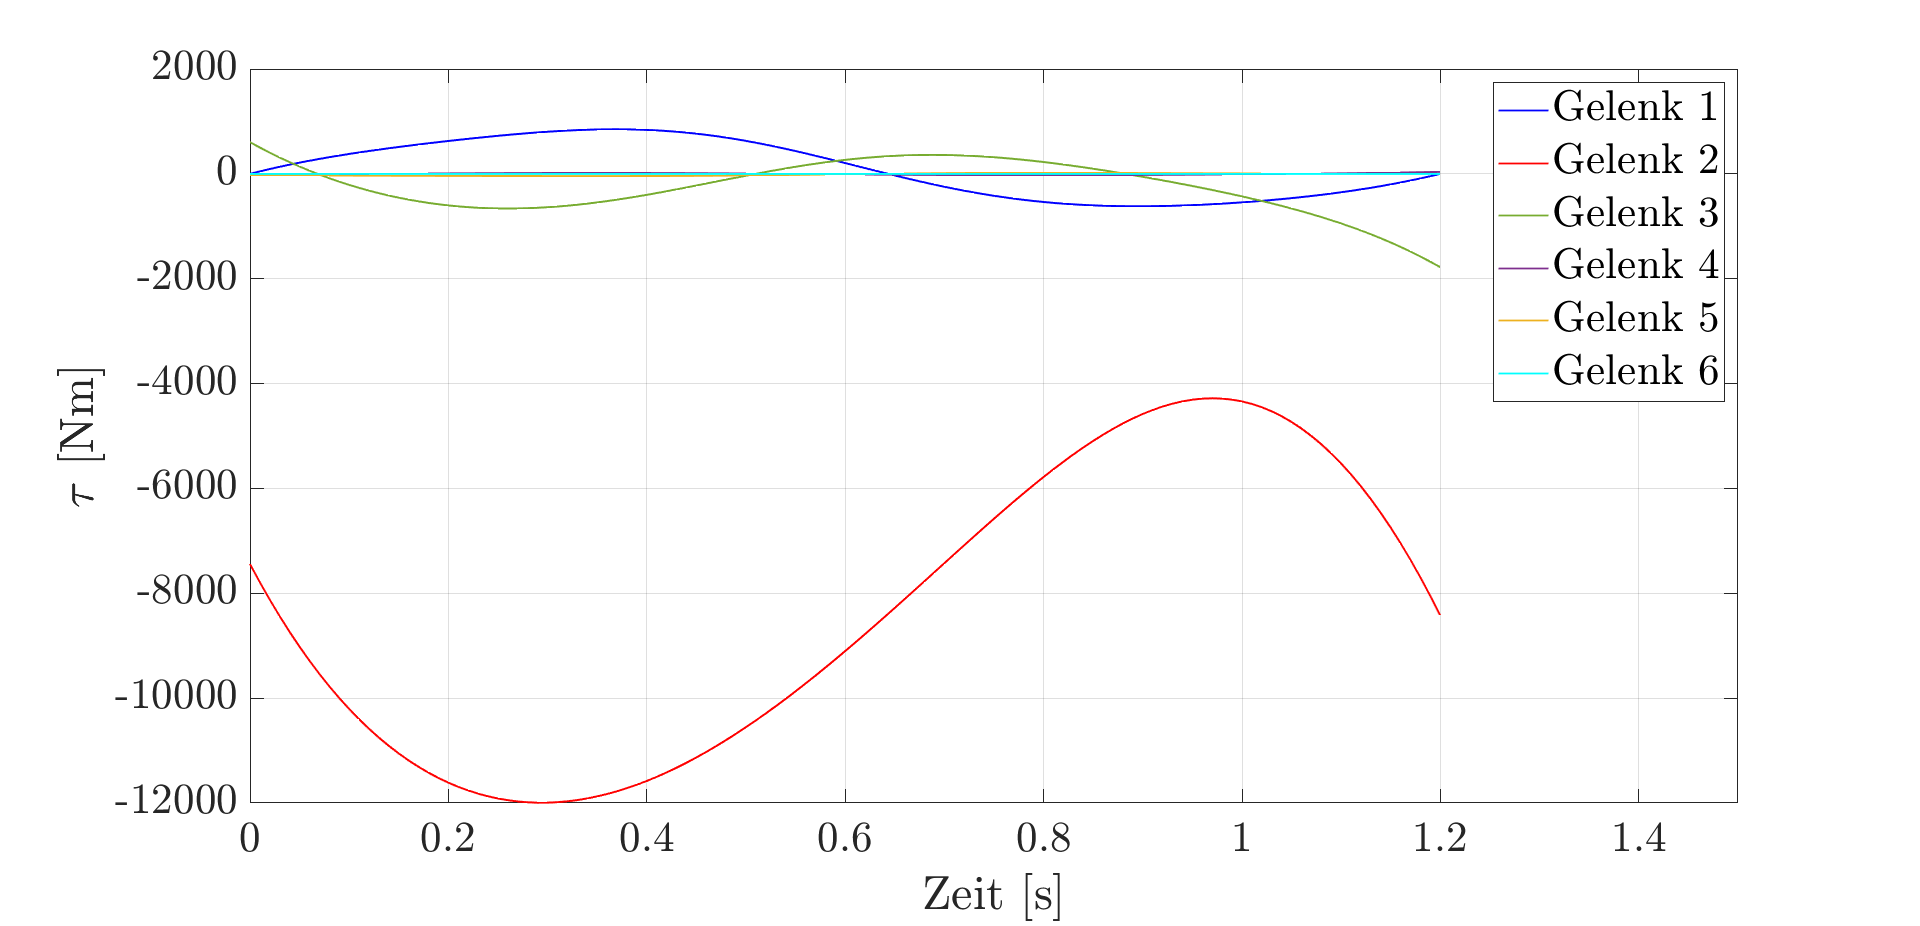
\includegraphics[width=1\linewidth]{images/taumat}
	\caption{Drehmomentverlauf simuliert}
	\label{fig:taumat}
\end{figure}
%
\begin{figure}[tbph]
	\centering
	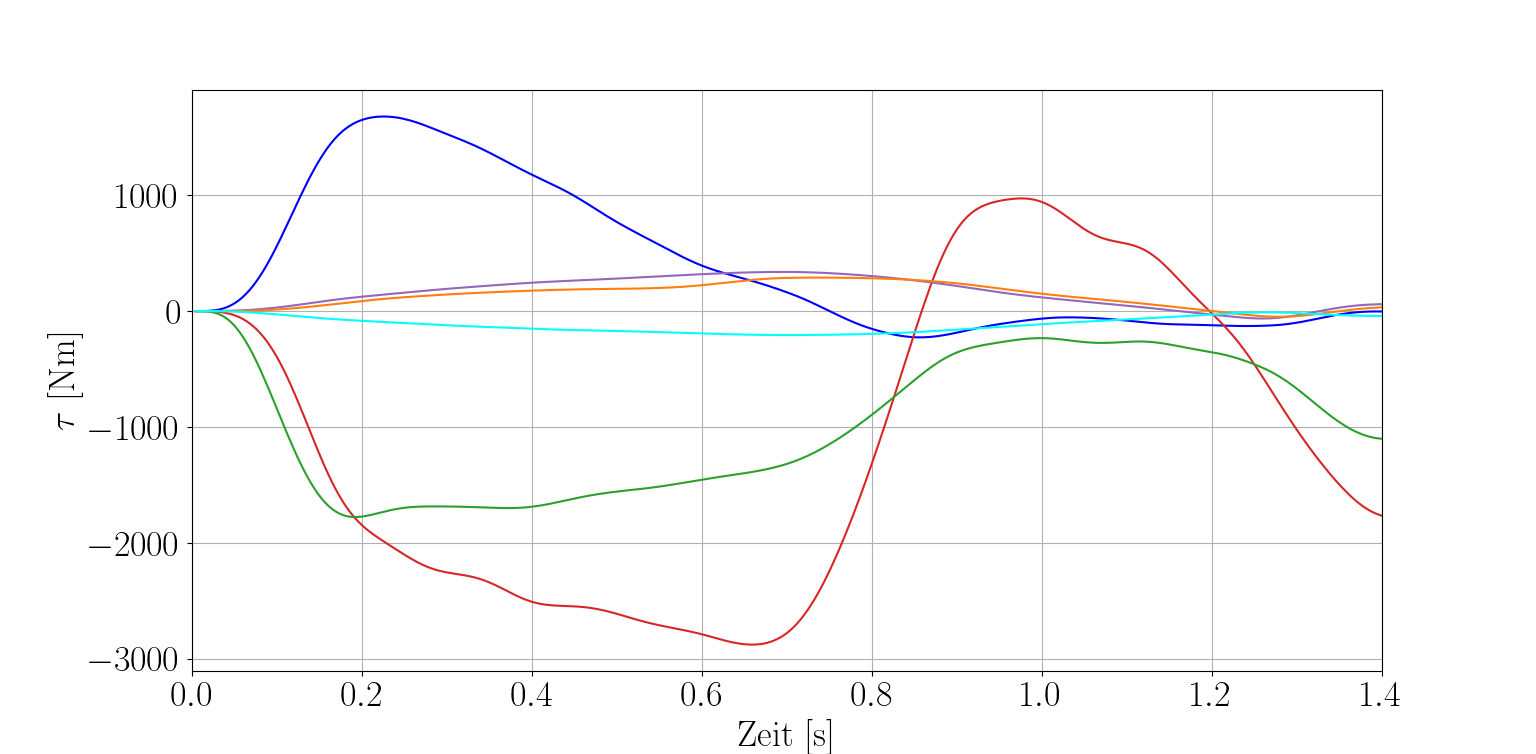
\includegraphics[width=1\linewidth]{images/tau}
	\caption{Drehmomentverlauf gemessen}
	\label{fig:tau}
\end{figure}
%
\begin{figure}[tbph]
	\centering
	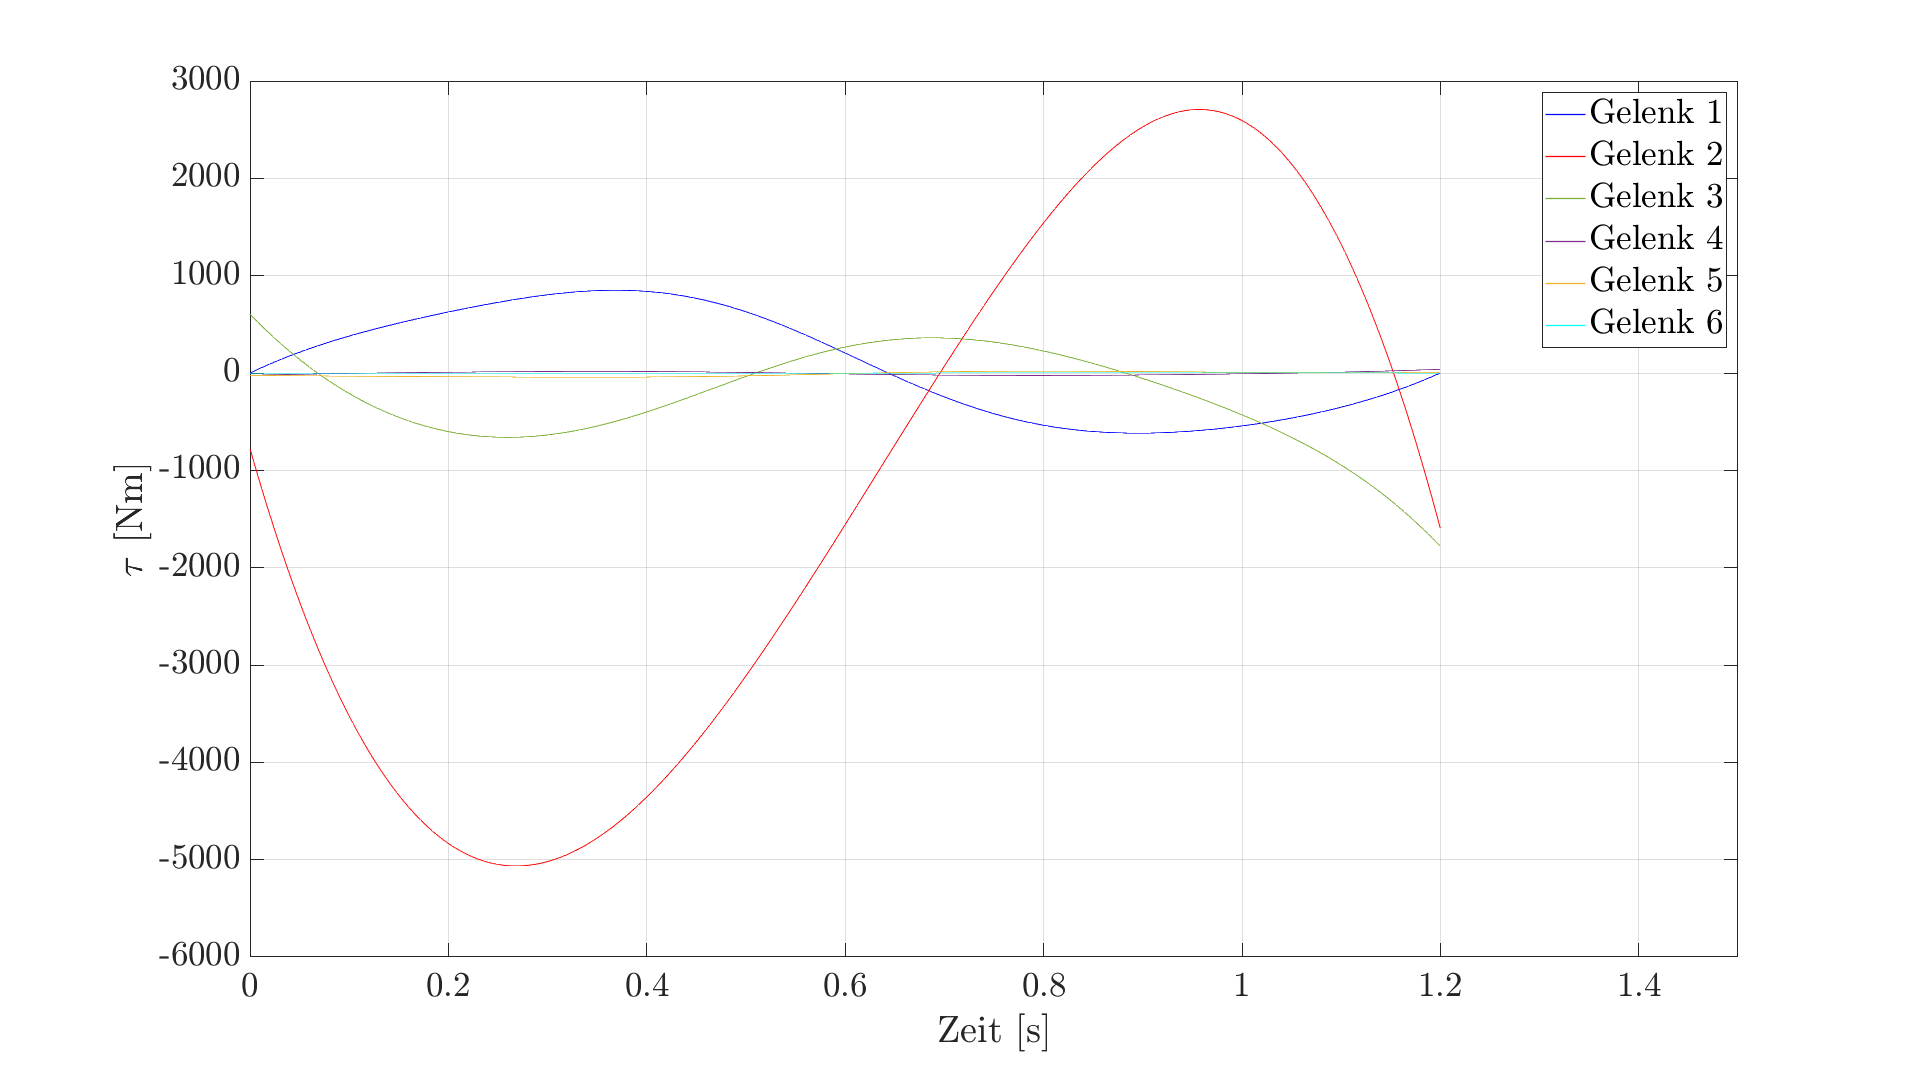
\includegraphics[width=1\linewidth]{images/taumat-fg}
	\caption{Drehmomentverlauf inkl. Gewichtsausgleich simuliert}
	\label{fig:taumat-fg}
\end{figure}
%
\begin{figure}[tbph]
	\centering
	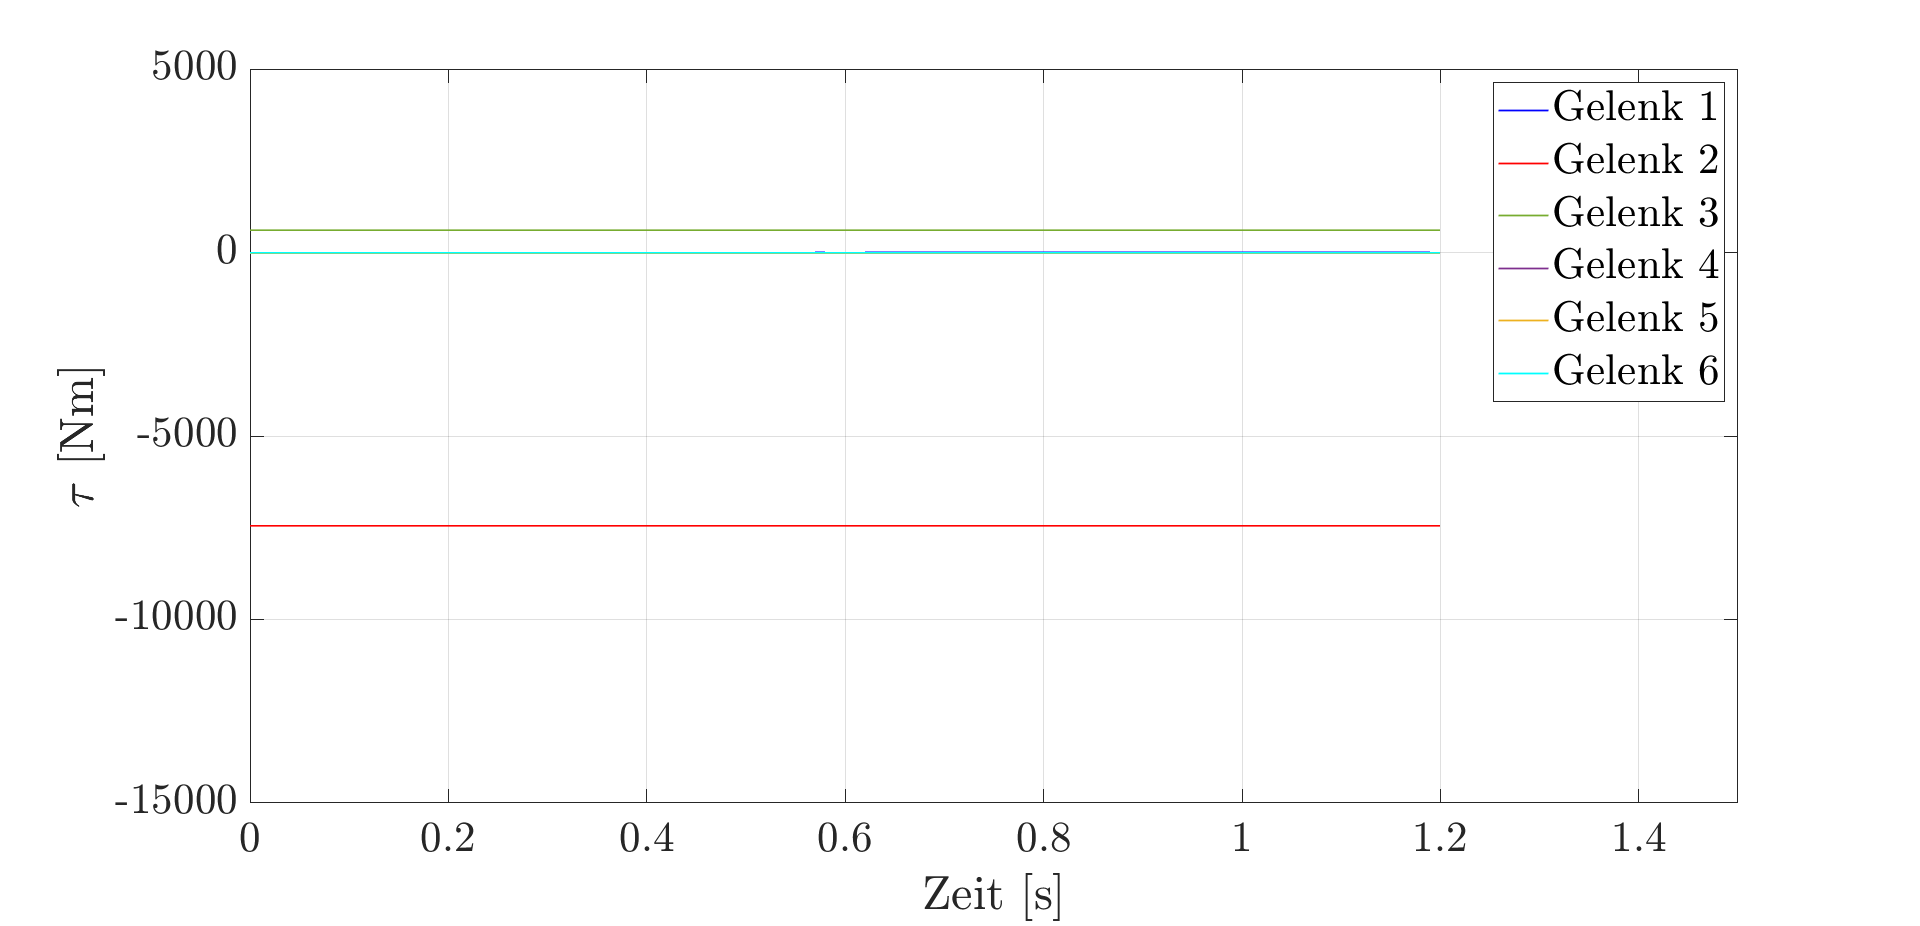
\includegraphics[width=1\linewidth]{images/Gewichtskraft}
	\caption{Anteil der Gewichtskraft an den Drehmomenten in der Startposition}
	\label{fig:gewichtskraft}
\end{figure}
%








\begin{figure}[tbph]
	\centering
	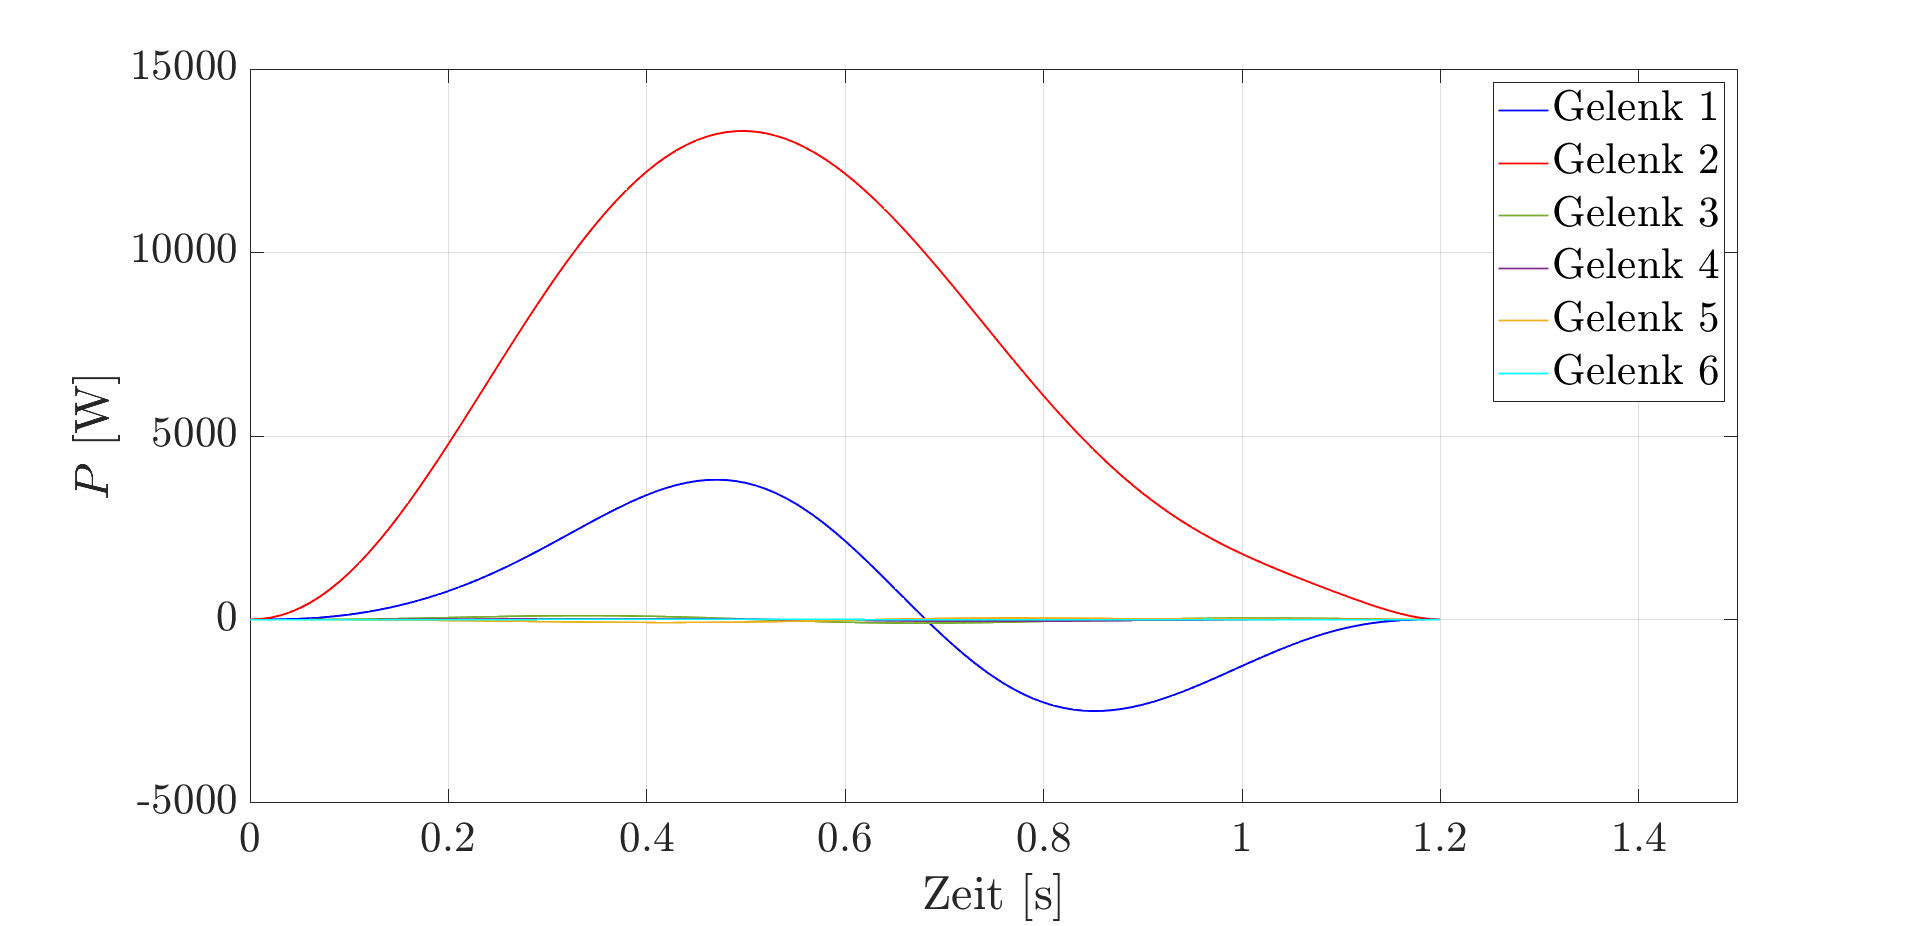
\includegraphics[width=1\linewidth]{images/pmat}
	\caption{mechanische Leistung simuliert}
	\label{fig:pmat}
\end{figure}
\begin{figure}[tbph]
	\centering
	\includegraphics[width=1\linewidth]{images/p}
	\caption{mechanische Leistung gemessen}
	\label{fig:p}
\end{figure}






\subsection{Schlussfolgerung}



Zeit


%%%%%%%%%%%%%%%%%%%%%%%%%%%%%%%%%%%%%%%%%%%%%%%%%%%%%%%%%%%%%%%%%%%%%%%%%%%%%%%%%%%%%%%%%%%
\section{Validierung der Optimierungsergebnisse}
Ziel ist die Energieeinsparung auf Basis des optimierten Via-Punkts am realen System zu validieren. Die Untersuchung verfolgt den Anspruch, dass identifizierte Einsparungen über die Laborumgebung hinaus in der industriellen Praxis erzielt werden können. Dazu werden  Einzelbewegungen der Bewegungsart PTP betrachtet, welche in nahezu jedem Programm das Verfahren in die Grundstellung oder auf eine Vorpositionen abbilden. Exemplarisch wird die Fahrt von der Grundstellung auf den ersten Prozesspunkt im Fertigungsprogramm $Kleben-Seitenwand$ (Bewegung Eins), sowie die Bewegung vom letzten Prozesspunkt zurück in die Grundstellung optimiert (Bewegung Zwei). Neben der Energieeinsparung wird auch die Verfahrzeit des Roboters auf der neuen Bewegungsbahn analysiert.
%
\subsection{Durchführung}
%Versuchsbeschreibung
%Definition von Start- und Zielpunkt
%Berechnung der Initialbahn durch die KR C
%Berechnung der Startviapunkte
\subsection{Ergebnisse}
\begin{figure}[tbph]
	\centering
	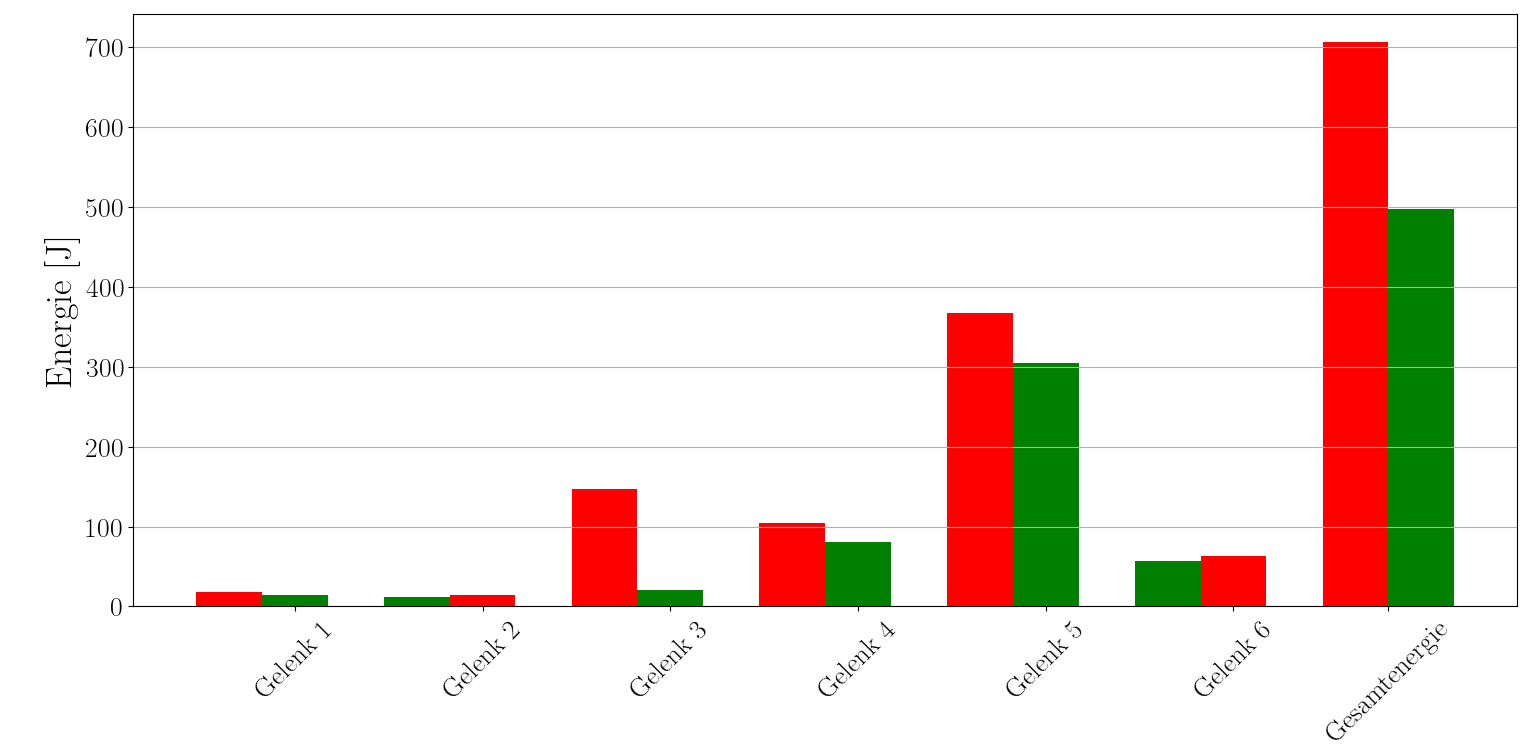
\includegraphics[width=1\linewidth]{images/e_down500}
	\caption{Energieverbrauch Bewegung Eins}
	\label{fig:edown500}
\end{figure}
\begin{figure}[tbph]
	\centering
	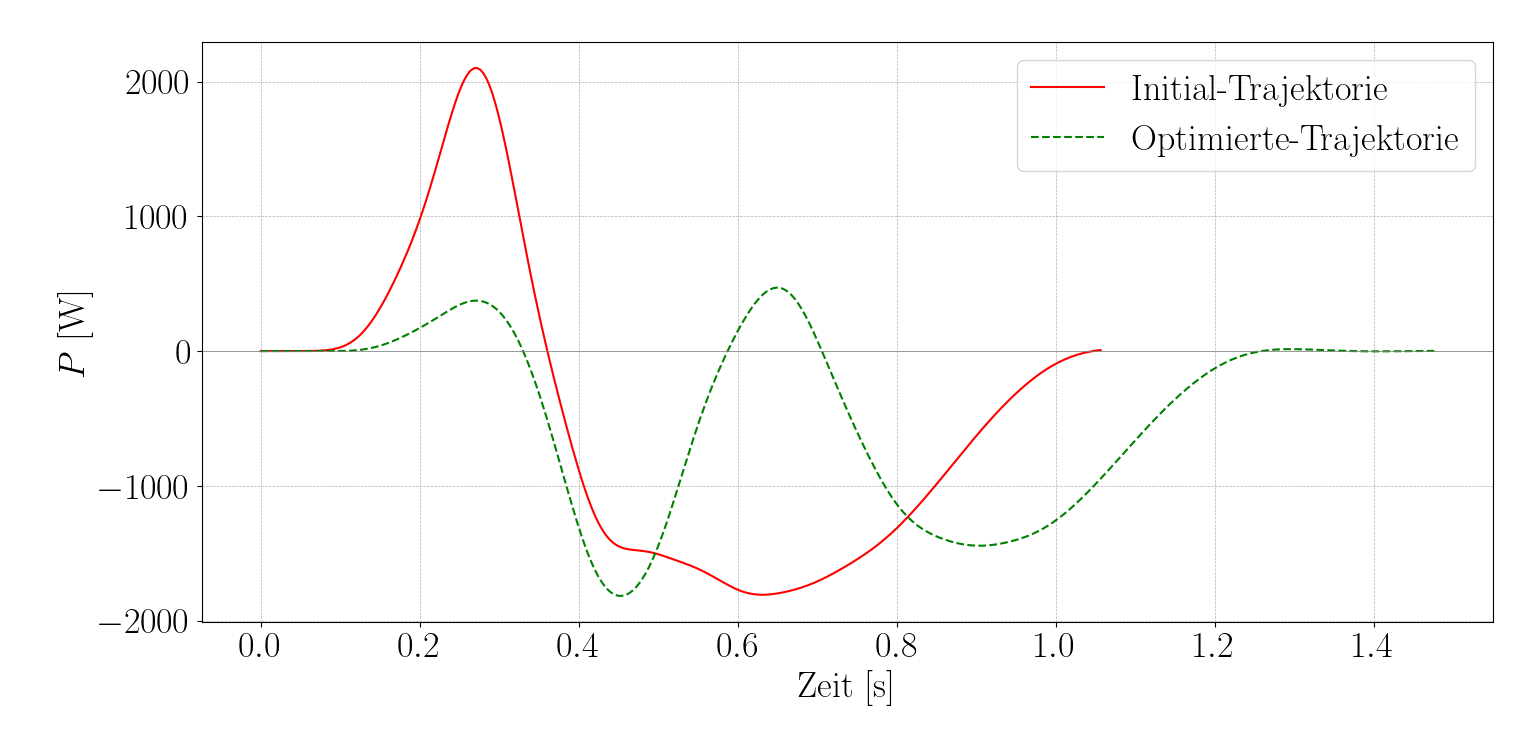
\includegraphics[width=1\linewidth]{images/P_down}
	\caption{Leistungsaufnahme Bewegung Eins}
	\label{fig:pdown}
\end{figure}
\begin{figure}[tbph]
	\centering
	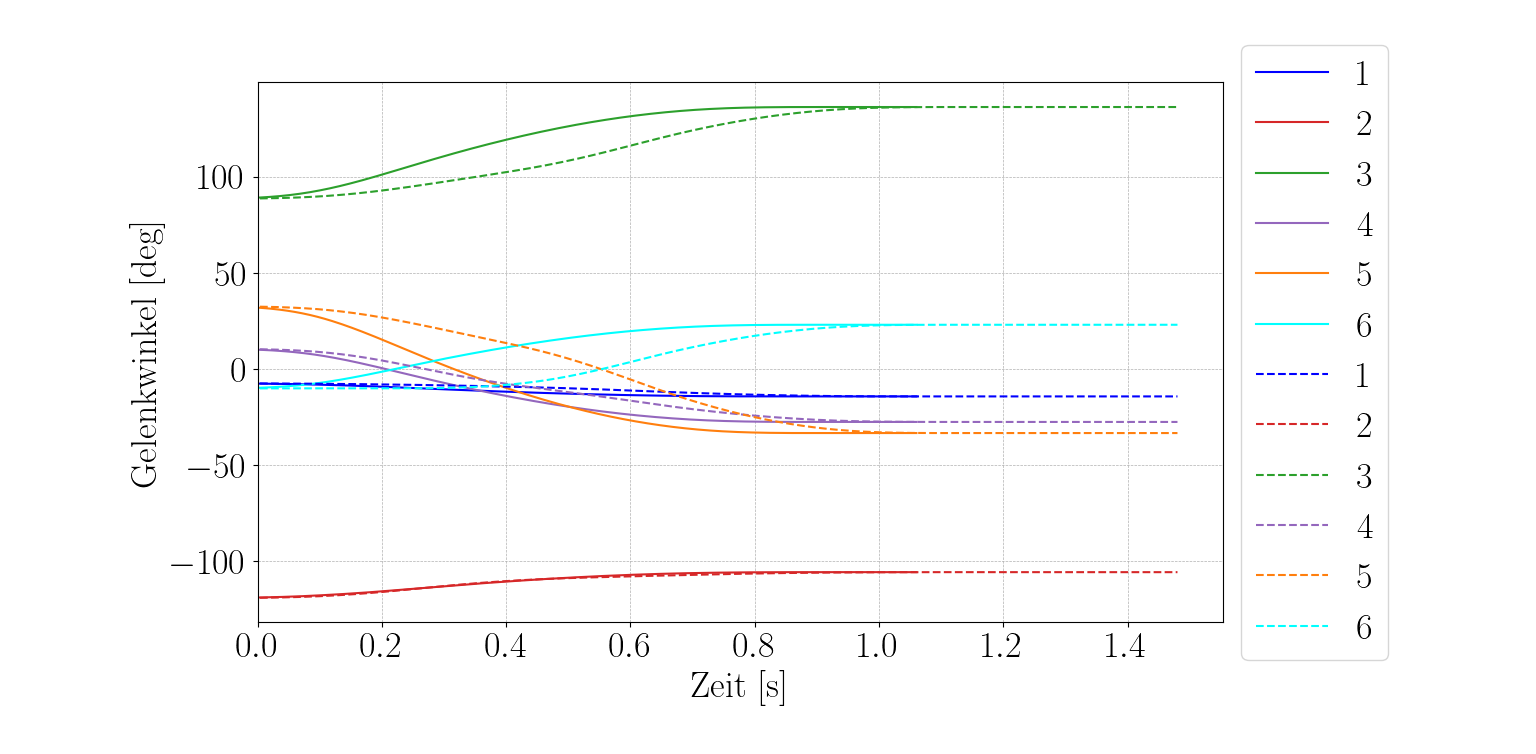
\includegraphics[width=1\linewidth]{images/aiposdown}
	\caption{Gelenkwinkel Bewegung Eins}
	\label{fig:aiposdown}
\end{figure}
\begin{figure}[tbph]
	\centering
	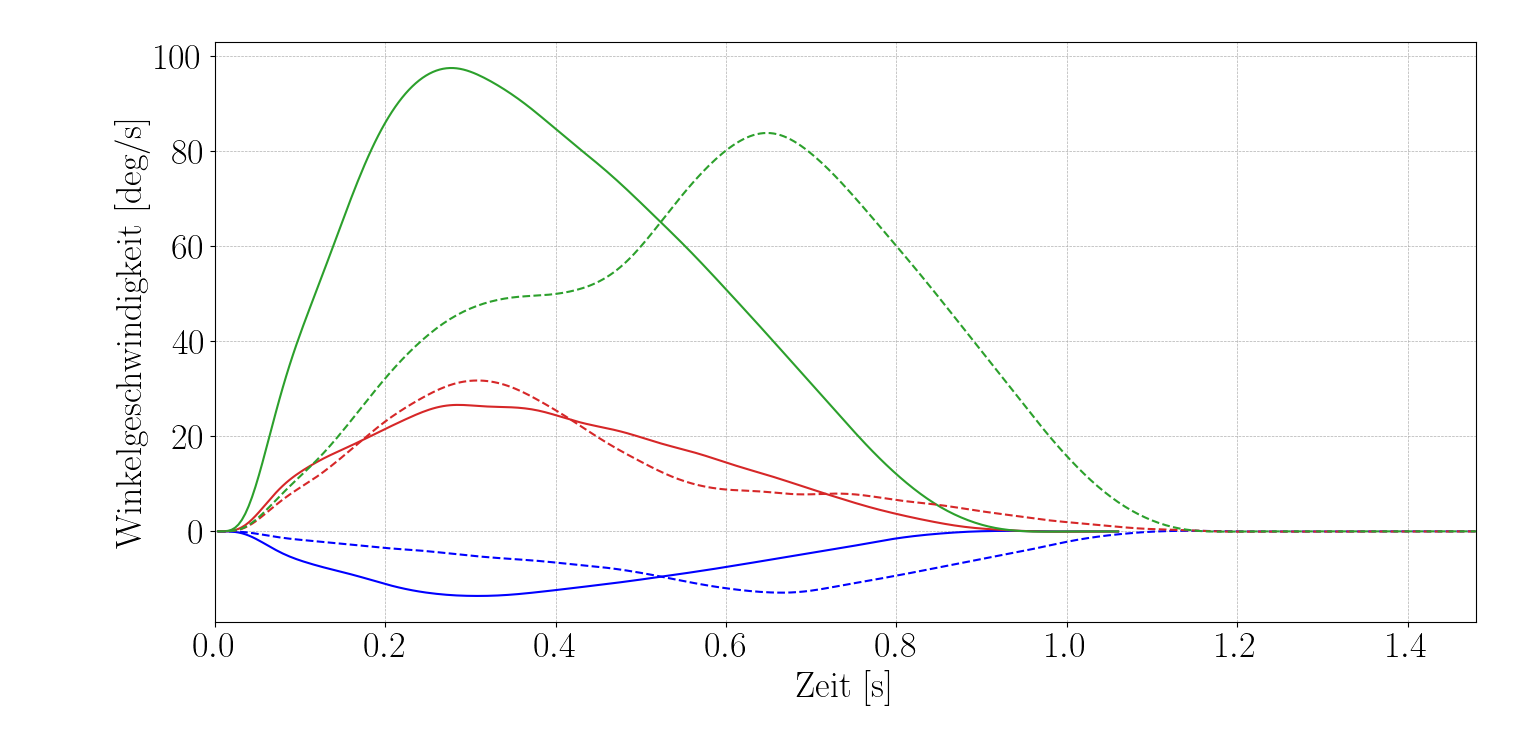
\includegraphics[width=1\linewidth]{images/velposdown1}
	\caption{Winkelgeschwindigkeit in den Gelenken 1-3 Bewegung Eins}
	\label{fig:velposdown1}
\end{figure}
\begin{figure}[tbph]
	\centering
	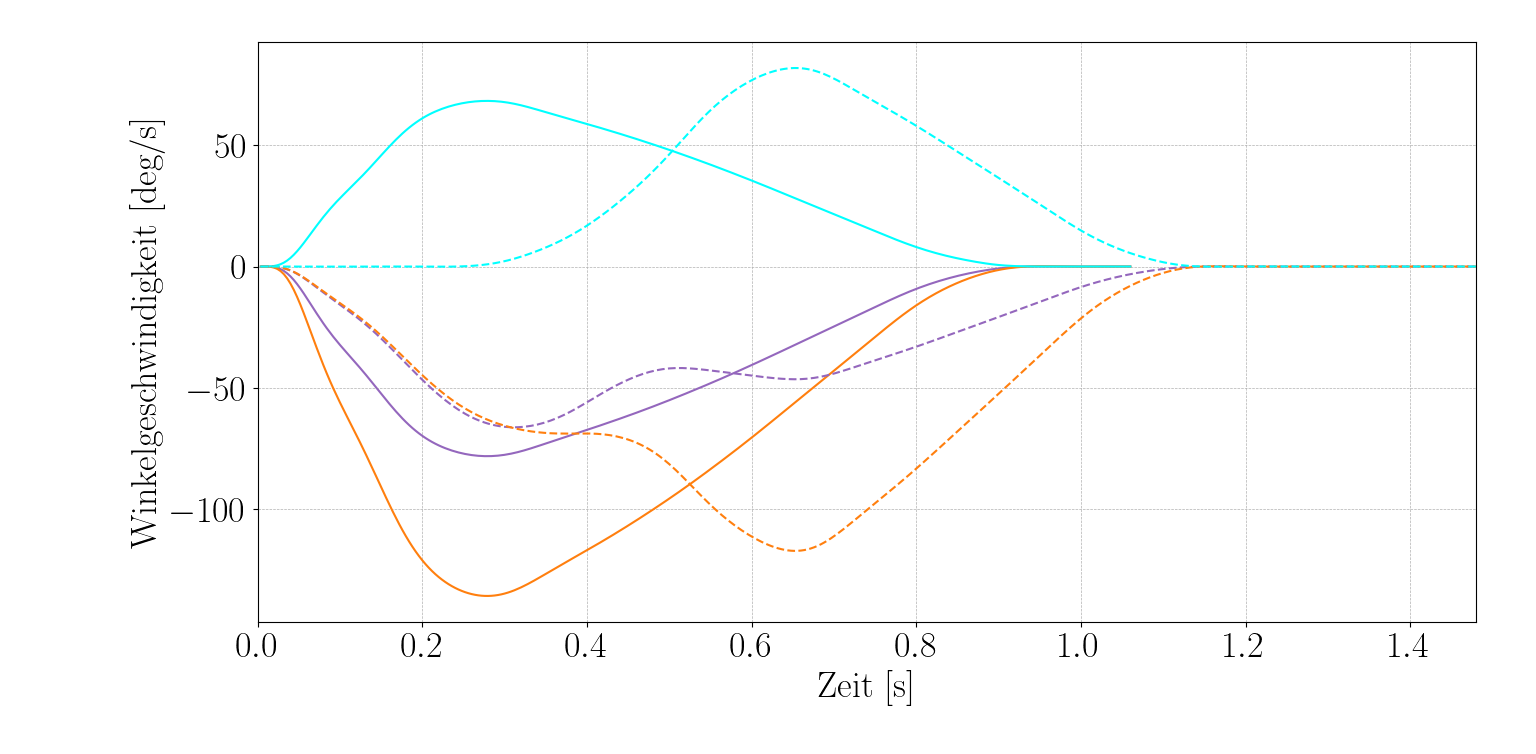
\includegraphics[width=1\linewidth]{images/velposdown2}
	\caption{Winkelgeschwindigkeit in den Gelenken 4-6 Bewegung Eins}
	\label{fig:velposdown2}
\end{figure}
\begin{figure}[tbph]
	\centering
	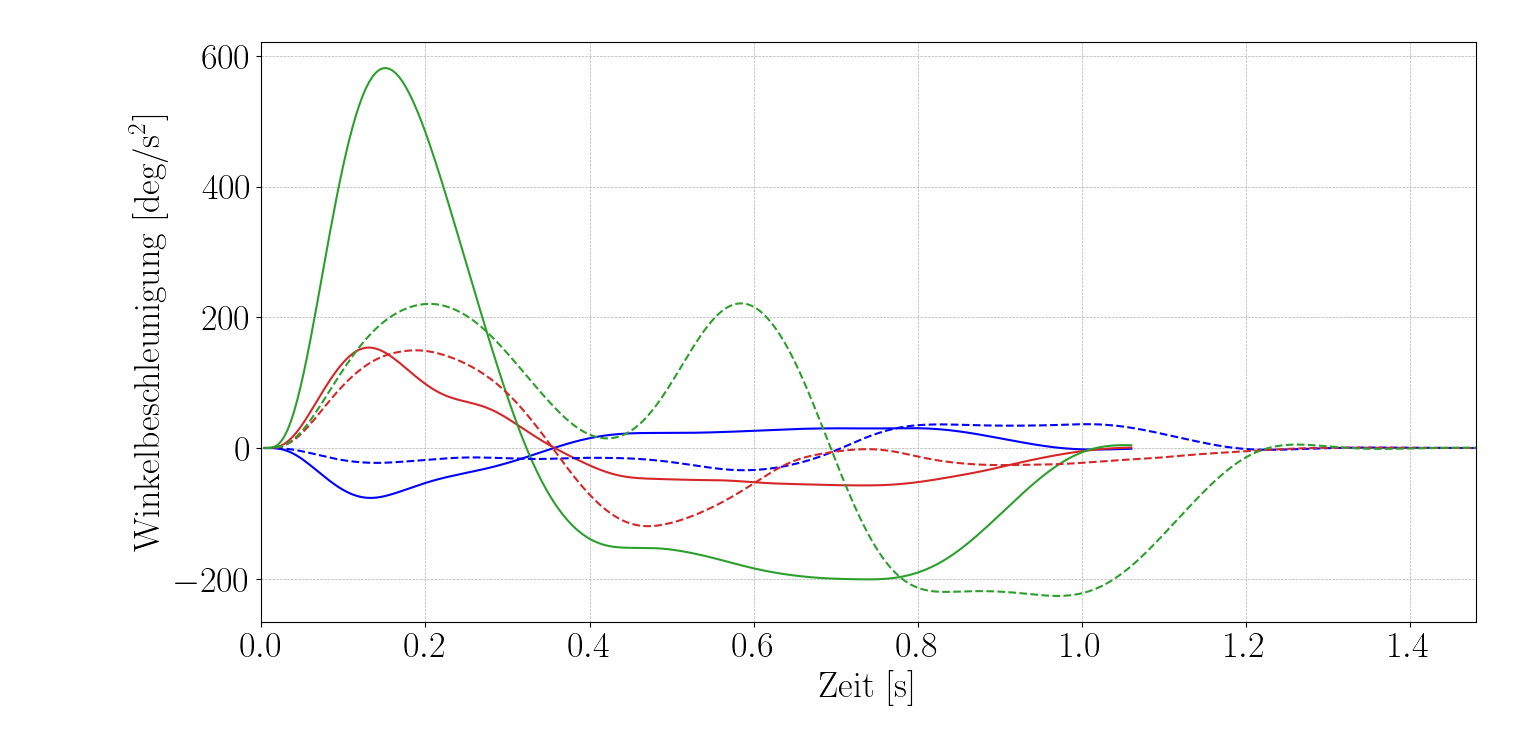
\includegraphics[width=1\linewidth]{images/accdown1}
	\caption{Winkelbeschleunigung in den Gelenken 1-3 Bewegung Eins}
	\label{fig:accdown1}
\end{figure}
\begin{figure}[tbph]
	\centering
	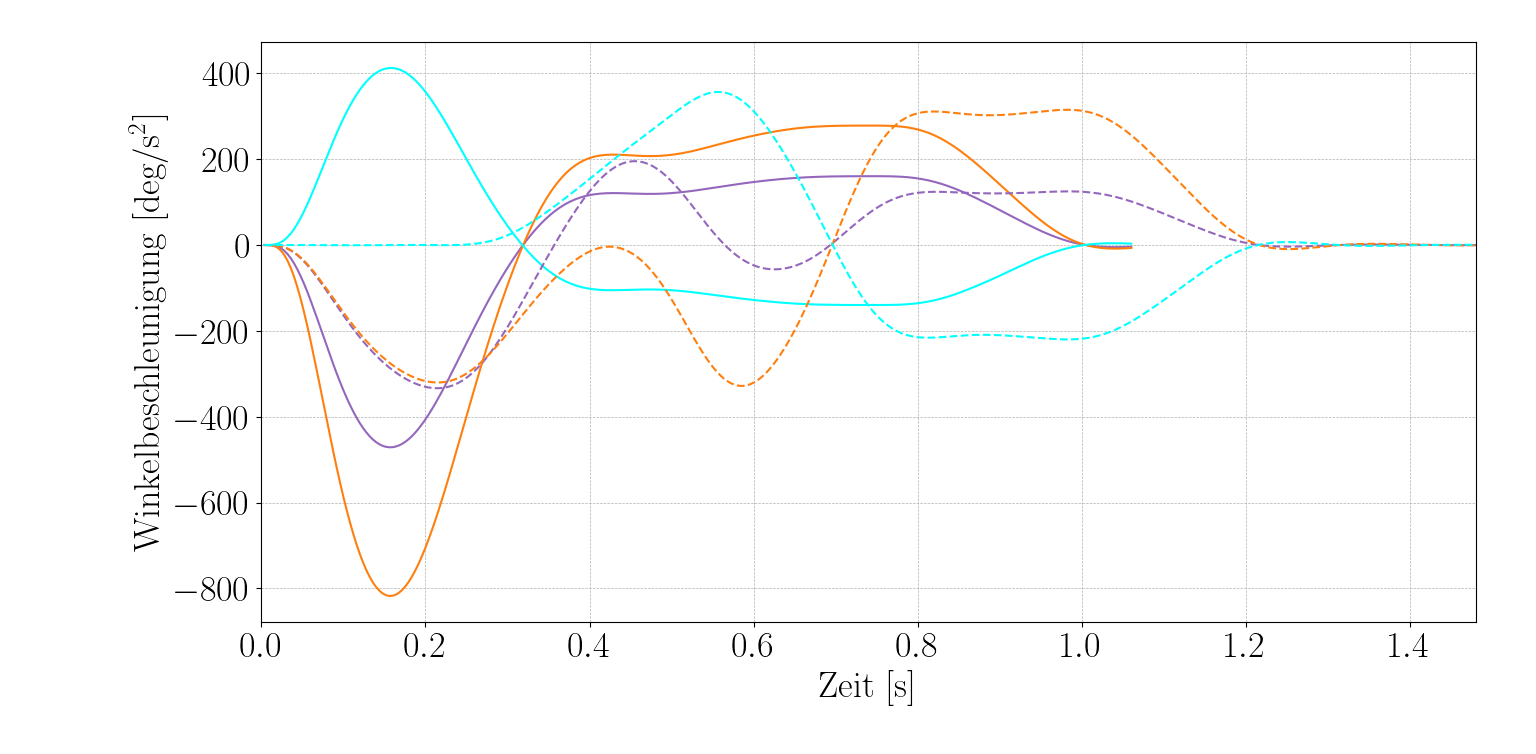
\includegraphics[width=1\linewidth]{images/accdown2}
	\caption{Winkelbeschleunigung in den Gelenken 4-6 Bewegung Eins}
	\label{fig:accdown2}
\end{figure}
%
%
%
%
\begin{figure}[tbph]
	\centering
	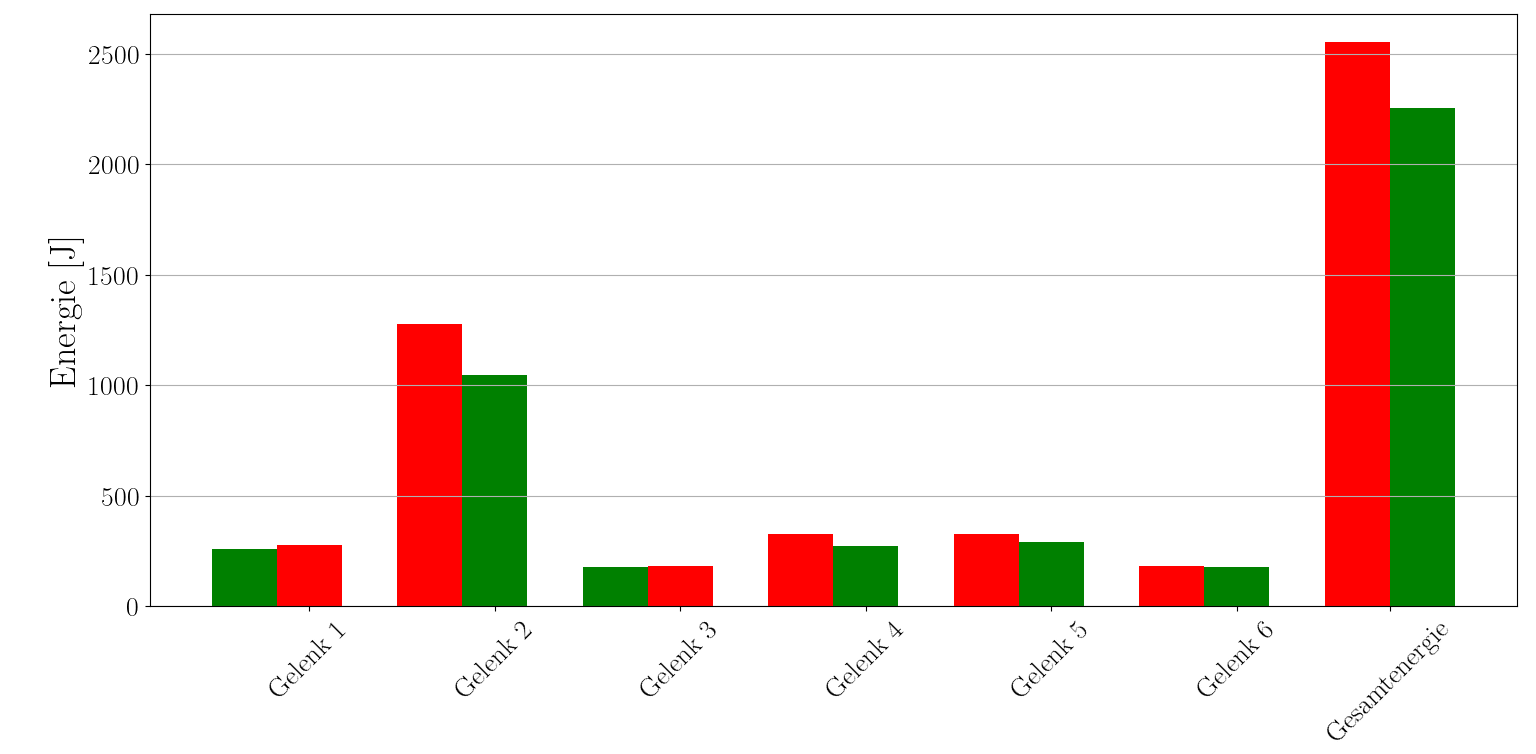
\includegraphics[width=1\linewidth]{images/e_up500}
	\caption{Energieverbrauch Bewegung Zwei}
	\label{fig:eup500}
\end{figure}
\begin{figure}[tbph]
	\centering
	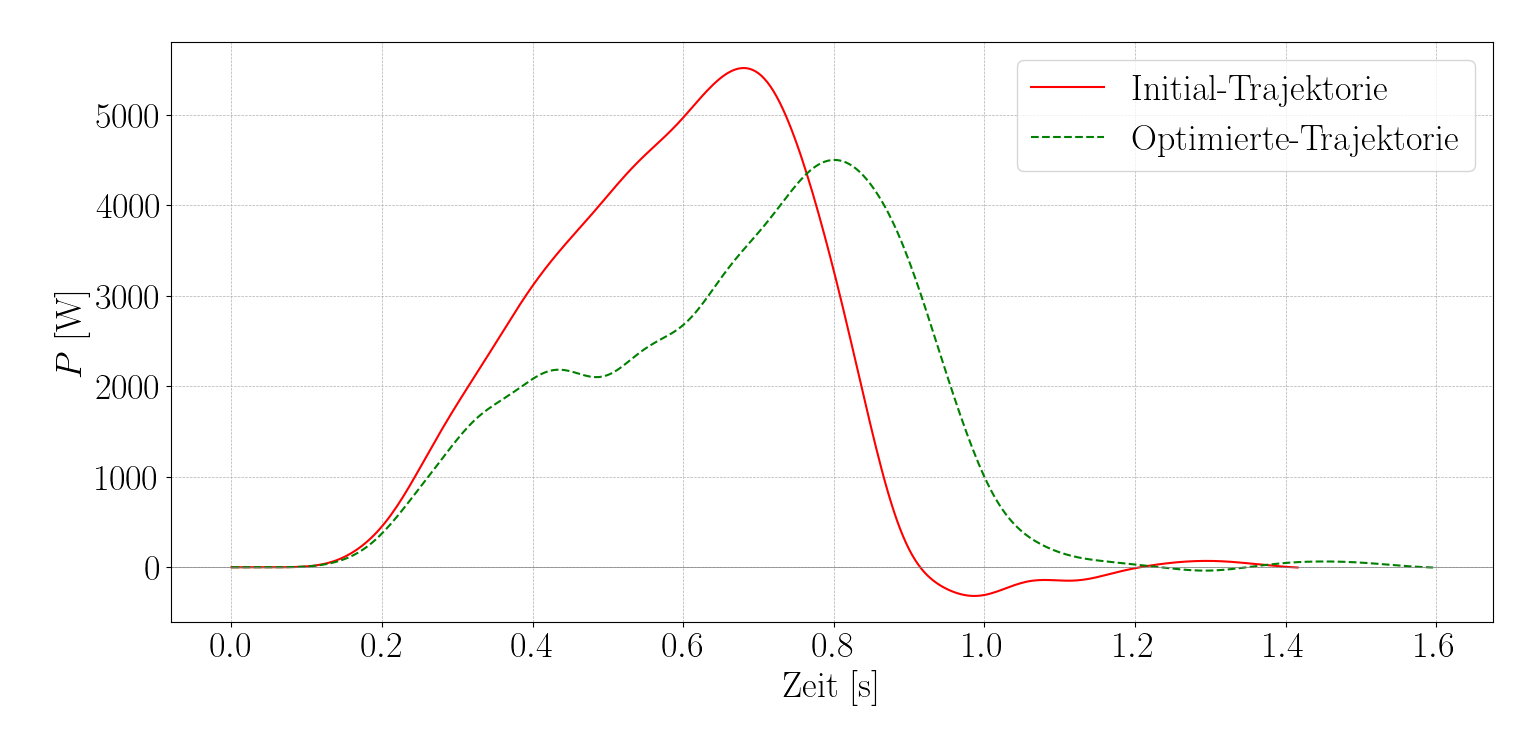
\includegraphics[width=1\linewidth]{images/P_up}
	\caption{Leistungsaufnahme Bewegung Zwei}
	\label{fig:pup}
\end{figure}
\begin{figure}[tbph]
	\centering
	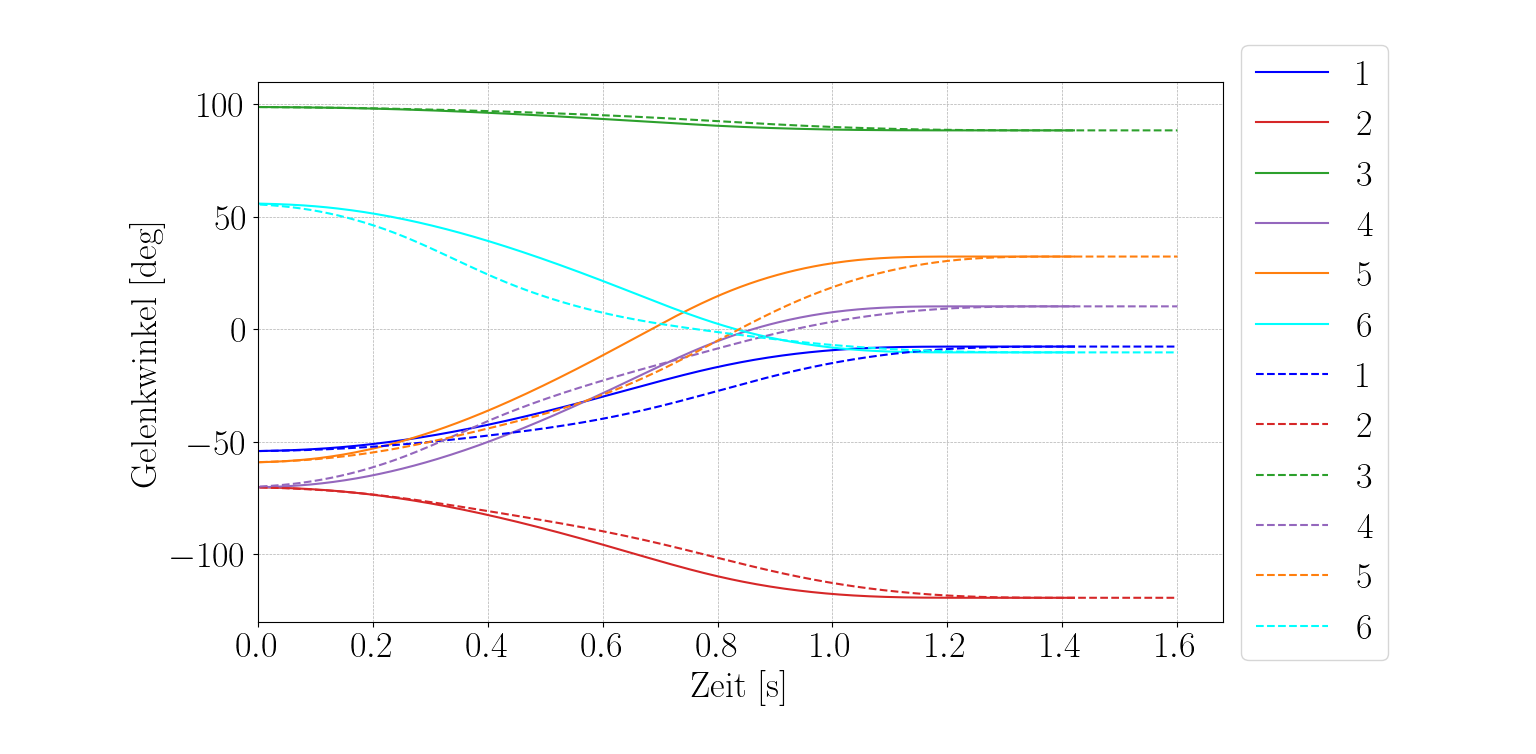
\includegraphics[width=1\linewidth]{images/aiposup}
	\caption{Gelenkwinkel Bewegung Eins}
	\label{fig:aiposup}
\end{figure}
\begin{figure}[tbph]
	\centering
	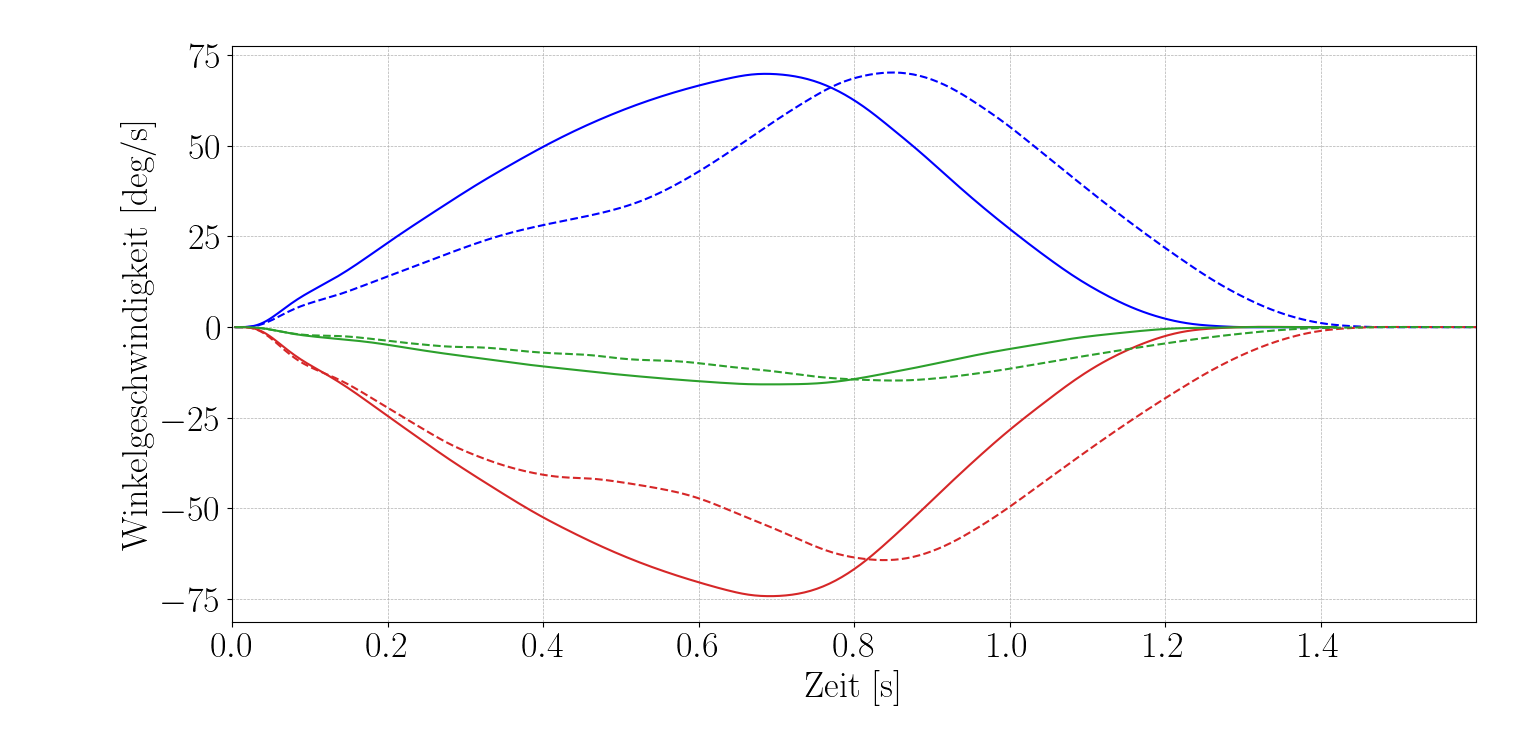
\includegraphics[width=1\linewidth]{images/velposup1}
	\caption{Winkelgeschwindigkeit in den Gelenken 1-3 Bewegung Zwei}
	\label{fig:velposup1}
\end{figure}
\begin{figure}[tbph]
	\centering
	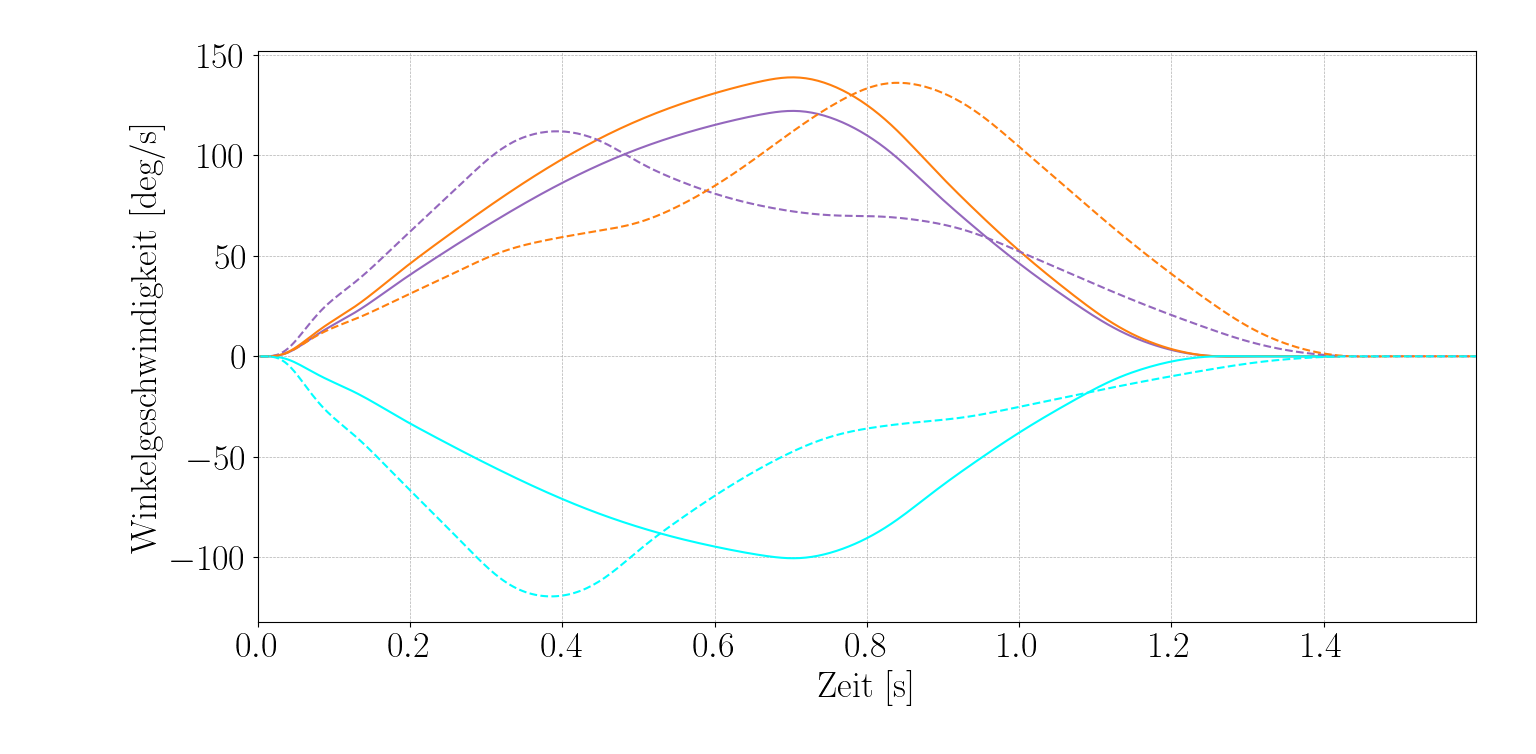
\includegraphics[width=1\linewidth]{images/velposup2}
	\caption{Winkelgeschwindigkeit in den Gelenken 4-6 Bewegung Zwei}
	\label{fig:velposup2}
\end{figure}
\begin{figure}[tbph]
	\centering
	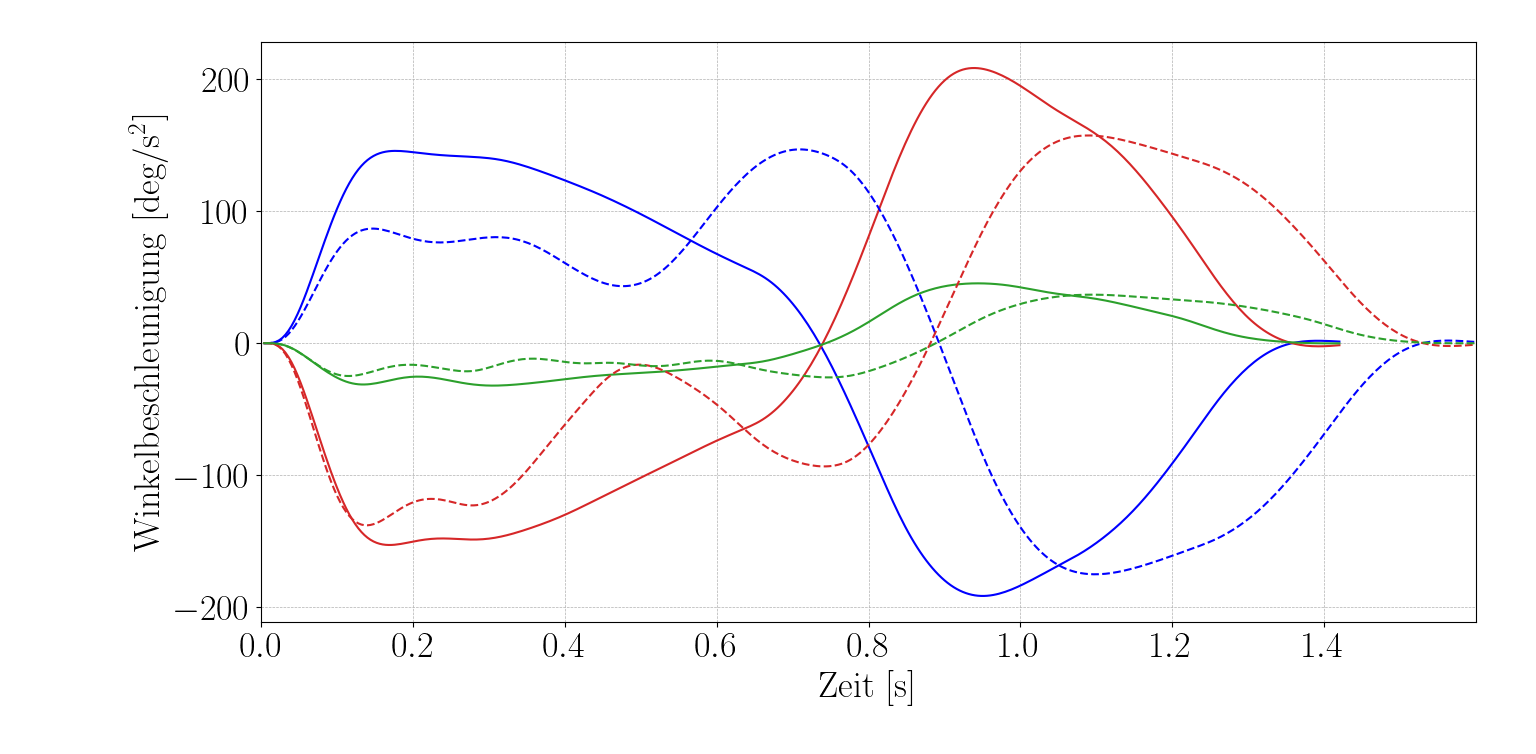
\includegraphics[width=1\linewidth]{images/accup1}
	\caption{Winkelbeschleunigung in den Gelenken 1-3 Bewegung Zwei}
	\label{fig:accup1}
\end{figure}
\begin{figure}[tbph]
	\centering
	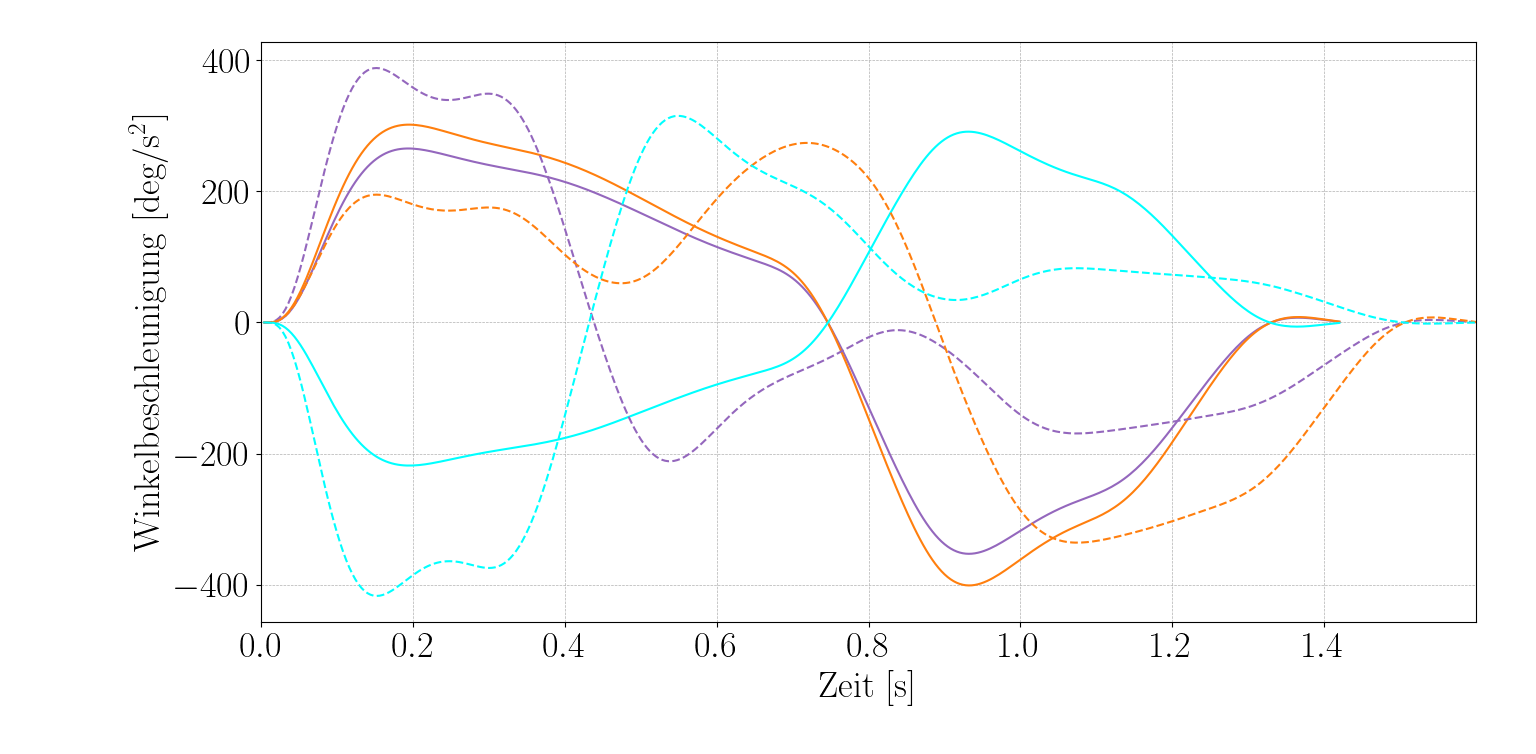
\includegraphics[width=1\linewidth]{images/accup2}
	\caption{Winkelbeschleunigung in den Gelenken 4-6 Bewegung Zwei}
	\label{fig:accup2}
\end{figure}

\subsection{Auswertung der Optimierungs- und Messergebnisse} 

%

%\subsection{Fehlerquellen}
%Temperatureinfluss auf die Reibung 